\chapter{TCP保活机制}

\section{引言}
许金 TCPAP的初学者会惊奇地发现,在一个空用的 TCP连接中不会有任何数据交换。也就是说,如果 TCP连接的双方都不向对方发送数据,那么 TCP 连接的两端就不会有任何
的数据交换。例如,在TCP协议中,没有其他网络协议中的轮询机制。这意味着我们可以启动一个客户端进程,与服务器端建立连接,然后离开儿个小时、几天、儿星期,甚至几个
月,而连接依然会保持。理论上,中间路由器可以崩溃和重启,数据线可以断开再连接,只要连接两端的主机没有被重新启动(或者更改 IP 地址),那么它们将会保持连接状态。

\begin{tcolorbox}
    上迷假设只是在特定情况下发生的。首先,客户端和服务器都没有实现应用层的非活动状态检测计时器,该计时器超时会导致任何一个应用进程的终止。其
    次,中间路由器不能保存连接的相关状态,例如一个NAT配置信息。某些特定採作中常常需要这些状态,而它们也会由于非活动状态而删除,或者由于系统故障而丢失。这些前提条件在现在的网络环境中是很难实现的。
\end{tcolorbox}

一些情况下,客户端和服务器需要了解什么时候终止进程或者与对方断开连接。而在另一些情况下,虽然应用进程之间没有任何数据交换,但仍然需要通过连接保持一个最小的数
据流。TCP保活机制就是为了解决上述两种情况而设计的。保活机制是一种在不影响数据流内容的情况下探测对方的方式。它是由一个保活计时器实现的。当计时器被激发,连接一端
将发送一个保活探测(简称保活)报文,另一端接收报文的同时会发送一个 ACK 作为响应。

\begin{tcolorbox}
    保活机制并不是TCP规范中的一部分。对此主机需求RFC [RFC1122] 给出了3个理由。(1)在出现短暂的网络错误的时候,保活机制会使一个好的连接断
    开;(2)保活机制会占用不必要的带宽;(3)在按流量计费的情况下会在互联网上花掉更多的钱。然而,大部分的实现都提供了保活机制。
\end{tcolorbox}

TCP 保活机制存在争议。许多人认为,如果需要,这一功能也不应在 TCP 协议中提供,而应在应用程序中实现。另一种观点认为,如果许多应用程序中都需要这一功能,那么在
TCP 协议中提供的话就可以使所有的实现都包含这一功能。保活机制是一个可选择激活的功能。它可能会导致一个好的连接由于两端系统之间网络的短暂断开而终止。例如,如果在中
间路由器崩溃并重新启动的时候保活探测,那么 TCP 协议将错误地认为对方主机已经崩溃。

保活功能一般是为服务器应用程序提供的,服务器应用程序希望知道客户主机是否崩遗或离开,从而决定是否为客户端绑定资源。利用TCP 保活功能来探测离开的主机,有助
于服务器与非交互性客户端进行相对短时间的对话,例如,Web 服务器、POP 和 IMAP电子邮件服务器。而更多地实现长时间交互服务的服务器可能不希望使用保活功能,如sh 和
Windows 远程桌面这样的远程登录系统。

河以通过一个简单例子来说明保活功能的可用性,即用户利用 ssh(安全 shell)证程務录程序穿越 NAT 路由器登录远程主机。如果建立连接,并做了相关操作,然后在一天结東
时没有退出,而是直接关闭了主机,那么便会留下一个半开放的连接。在第13章中已经提到过,通过一个半开散的连接发送数据会返回一个重置信息,但那是来自正在发送数据的客
户端。如果客户端离开了,只剩下服务暑端的一个半开放的连接,而服务器又在等待客户缩发来的数据,那么服务器将会永远地等待下去。在服务器端探测到这种半开放的连接时,就
可以使用保活功能。

相反的情况下同样需要使用保活机制。如果用户没有关闭计算机,而是整个晚上保持连接,第二天可以继续使用,那么连接将连续几个小时处于空闲状态。在第7章中我们提到
过,大部分NAT 路由器包含超时机制。当连接在一段时间内处于非活动状态时,路由器格断开连接。如果 NAT 超时时限小于用户重新登录之前的几个小时,且 NAT不能探测到端主
机并确认它还处于活动状态,或者 NAT 路由器崩溃,那么该连接将被终止。为了避免这种情况的发生,用户可以配置 ssh,启动 TCP 保活功能。ssh 还能够使用应用程序管理的保话
功能。两种功能的行为模式不同,特别是安全性方面(参见17.3节了解细节)。

\section{描述}
保活功能在默认情况下是关闭的。TCP 连接的任何一端都可以请求打开这一功能。保话功能可以被设置在连接的一端、两端,或者两端都没有。有几个配置参数可以用来控制保活
功能的操作。如果在一段时间(称为保活时间,keepalive time)内连接处于非活动状态,开启保活功能的一端将向对方发送一个保活探测报文。如果发送端没有收到响应报文,那么经
过一个已经提前配置好的保活时间间隔(keepalive interval),将继续发送保活探测报文,直到发送探测报文的次数达到保活探测数(keepalive probe),这时对方主机将被确认为不可到
达,连接也将被中断。

保活探测报文为一个空报文段(或只包含1字节)。它的序列号等于对方主机发送的ACK 报文的最大序列号减1。因这一序列号的数据段已经被成功接收,所以不会对到达的
报文段造成影响,但探测报文返回的响应可以确定连接是否仍在工作。探测及其响应报文都不包含任何新的有效数据(它是“垃圾”数据),当它们丢失时也不会进行重传。[RFCI122]
指出,仅凭一个没有被响应的探测报文不能判断连接是否已经停止工作。这就是保活探测数参数需要被提前设置的原因。值得注意的是,一些 TCP 实现(大部分是早期的TCP 实现)
不会响应那些不包含“垃圾”数据的保活探测报文。

TCP保话功能工作过程中,开启该功能的一端会发现对方处于以下四种状态之一:
\begin{enumerate}
    \item 对方主机仍在工作,并且可以到达。对方的TCP响应正常,并且请求端也知道对方在正常工作。请求瑞将保活计时器重置(重新设定为保活时间值)。如果在计时器超时之前有应用程序通过该连接传输数据,那么计时器将再次被设定为保活时间值。
    \item 对方主机已经崩溃,包括已经关闭或者正在重新启动。这时对方的TCP 将不会响应。请求端不会接收到响应报文,并在经过保活时间间隔指定的时间后超时。超时前,请求端会持续复送探测报文,一其废送保活採删数指定次数的探测报文,如果请求端没有收到任何採测报文的响点,那么它将认为对方主机已经关闭,连接也将被断开。
    \item 客户主机崩溃并且已重启。在这种情况下,请求端会收到一个对其保活探测报文的响应,但这个响应是一个重置报文段,请求端将会断开连接。
    \item 对方主机仍在工作,但是由于某些原因不能到达请求端(例如网络无法传输,而且可能使用ICMIP 通知也可能不通知对方这一事实)。这种情况与状态2相同,因为 TCP 不能区分状态2与状态4,结果都是没有收到探测报文的响应。
\end{enumerate}

请求端不必担心对方主机正常关闭然后重启(不同于主机崩溃)的情况。当系统关机时,所有的应用进程也会终止(即对方的进程),这会使对方的TCP发送一个FIN。请求端接收
到FIN 后,会向请求瑞进程报告文件结束,并在检测到该状态后退出。

在第1种情况下,请求端的应用层不会觉察到保活探测的进行(除非请求端应用层激活保活功能)。一切操作均在 TCP 层完成,因此这一过程对应用层是透明的,直至第2、3、4种
情況中的某种情况发生。在这三种情况中,请求端的应用层将收到一个来自其 TCP 层的差错报告(通常请求端已经向网络发出了读操作请求,并且等待来自对方的数据。如果保活功能返
回了一个差错报告,则该差错报告将作为读操作请求的返回值返回给请求端)。在第2种情况下,差错是诸如“连接超时”之类的信息,而在第3种情况下则为“连接被对方重置”。第4
种情况可能是逢接超时,也可能是其他的错误信息。在下一节中我们将重点讨论这四种情况。

变量保活时间、保活时间间隔和保活探测数的设置通常是可以变更的。有些系统允许用户在每次建立连接时设置这些变量,还有一些系统规定只有在系统启动时才能设置(有的系
统两者皆可)。在 Linux 系统中,这些变量分别对应 sysctl 变量 \verb|net.ipv4.tcp_keepalive_time|、\verb|net.ipv4.tcp_keepalive_intvl|、\verb|net.ipv4.tcp_keepalve_probes|,默认设置是7200秒(2小时)、
75秒和9次探测。

在FreeBSD 和 Mac OS X 系统中,前两个变量对应 sysctl 变量 \verb|net.inet.tcp.keepidle| 和\verb|net.inet.tcp.keepintvl|,默认设置力7200秒(2小时)和75000毫秒(75秒)。这两个系统
还包含一个名为\verb|net.inet.tcp.always_keepalive|的布尔变量。如果这个变量被激活,那么即使应用程序没有请求,所有 TCP 连接的保活功能都会被激活。探测次数被设定为固定值8
(FreeBSD 系统)或9(Mac OS X 系统)。

在 Windows 系统中,可通过在系统键值下修改注册表项来设置变量:
\begin{verbatim}
    HKLM\SYSTEM\CurrentControlSet\Services\Tcpip\Parameters
\end{verbatim}

KeepAliveTime 保活时间默认为7200 000毫秒(2小时),KeepAliveInterval(保活时间间隔)默认为1000毫秒(1秒)。如果10个保活探测报文都没有响应,Windows 系统将终止
连接。

值得注意的是,[RFC1122] 明确给出了用户使用保活功能的限制。保活时间值必须是可配置的,而且默认不能小于2小时。此外,除非应用层请求开启保活功能,否则不能使用该
功能(而如果 \verb|net.inet.tcp.always_keepalive| 变量被设置时会违反这一限制)。没有经过应用层的请求,Linux 系统不会提供保活功能,但是一个特殊库会被预先栽入(即在载人普通共享
库之前),从而实现该功能[LKAJ。

\subsection{保活功能举例}
现在详细讨论上一节提到的第2、3、4种情况,我们将在使用保活机制的前提下观察数据包的交换。第1种情况的操作将在观察其他几种情况的过程中涉及。
\subsubsection{另一端崩潰}
我们想了解当服务器主机崩溃且没有重新启动时的过程。为了模拟这种情况,我们需要进行以下几个步骤:
\begin{enumerate}
    \item 利用Windows 客户端上的 regedit 程序,修改注册表键值,将 KeepAliveTime 设置7000毫秒(7秒)。设置新的值,可能需要系统重新启动。
    \item 在Windows客户端和一个已经开启 TCP 保活功能的Linux服务器之间建立 ssh 连接。
    \item 确保数据可以通过该连接传输。
    \item 观察客户端的 TCP每7秒发送一个保活数据包,并且这些数据包都可以被服务器TCP 接收到。
    \item 保持服务器端的网线断开。这时客户端会认为服务器主机已经崩溃。
    \item 我们预计,在确认连接断开之前,客户端会发送10个间隔为1秒的保活探测报文。
\end{enumerate}

这里是客户端的交互输出结果:
\begin{verbatim}
    C: \> ssh -0 TCPKeepAlive=yes
10.0.1.1
(password prompt and login continues)
Write ralled:
Connection
reset by peer (about 15 seconds after disconnect)
\end{verbatim}

图17-1是利用 Wireshark工具的显示结果。在这个例子中,连接已经被建立。Wireshark首先输出一个没有被识别的保活报文(数据包1)。此时,Wireshark 还没有足够的数据包来
处理,不能发现数据包1中的序列号小于接收端窗口的左边界,因此不能判断数据包1是一个保活报文。数据包2中包含一个ACK 号,它可以使 Wireshark 对后续数据包中的序列号
进行适当的处理。

这一连接大部分由保活报文和对应的响应报文组成。数据包1、3、5、7、14、16、18、20以及22~31都是保活报文。数据包2、4、6、8、15、17、19、21是这些报文相应的响应。
如果保活报文得到响应,那么客户端将每隔7秒发送一次。而当保活报文没有被响应时,发送方将会根据 KeepAlivelnterval 设定的默认值,转变为每隔1秒发送一个保活报文。这一情
况发生在62.120s时刻,也就是第23个数据包发送时。发送方共发送了10个没有被响应的保活报文(数据包 22~31)。在这之后,客户端会断开连接,发送最后的重置报文段(数据
包32),但不会收到对方的任何响应。当连接断开时,用户将收到下面一段输出信息:
\begin{verbatim}
    Write failed: Connection reset by peer
\end{verbatim}
很明显连接已经断开,但是这种方式并不完全准确。事实上的确是发送端将连接断开的,但是发送端是基于缺少接收端的响应才做出这一判断的。

除了利用了保活机制之外,这一连接还有一些其他有趣的功能,这里做简要说明。首先,服务器使用了 DSACK 机制(第14章)。每一个ACK 包含一个序列号区间,为之前接
收到的序列号范围。其次,在26.09s时刻,有一个很小比特的数据交换。这个数据只代表了一个键盘键的按下。它被发送给服务器,服务器对其进行确认并回显。由于这一数据被加
密,导致该数据包中的用户数据大小为48字节(第18章)。

有趣的是,回显的数据被发送了两遍。可以看到11号包为回显数据包,但是它没有被立即响应。回想一下第14章,Linux 系统 RTO 至少为200毫秒。这里我们可以看到,Linux
服务器在 200毫秒之后重传了该数据,这次传输很快得到了客户端的响应。因为网络中无拥塞发生,所以基本不可能出现11号包丢失的情况。由于客户端的延迟响应,Linux 服务器
进行了假重传。这种情况类似于第15 章讨论过的Nagle算法与延时ACK 的关系。从结果上看,这里发生了不必要的200毫秒延迟。

\begin{figure}[!htb]
    \centering
	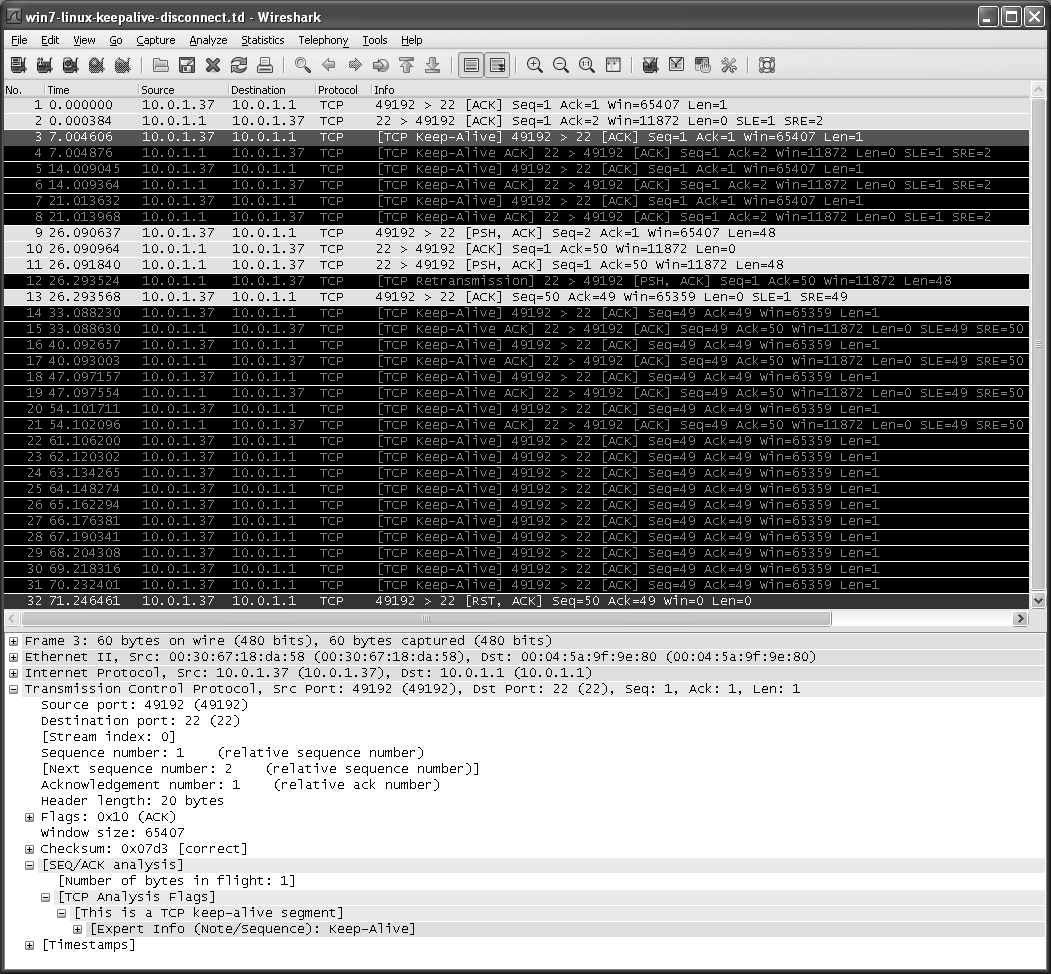
\includegraphics[width=1\textwidth]{imgs/17/17-1.png}
	\caption{连接空闲之后,TCP保活报文每间隔7秒发送一次。每一个报文中包含一个小于已被确认觉据的序列号。当网线断开1分钟后,后续的保活报文就不会收到响应。客户端会发送10次
    保活报文,如果都没有响应会将连接断开。断开连接时,客户端会向服务器发送重置报文段(服务器不会接收到)。这个例子还说明了服务器使用了 DSACK 机制,客户端的延迟响应会
    导致假重传}
\end{figure}

\subsubsection{另一端崩溃并已重新启动}
在这个例子中,我们需要观察当对方主机崩溃并且重启时会发生什么。这一次我们把KeepAliveTime 设置为120000毫秒(2分钟),其他的初始设置与前面的例子相同。我们建
立一个连接,然后等待2分钟,客户端会发送一个保活消息并成功接收到相应的响应。之后我们将服务器端的网络断开,并将服务器重新启动,最后将它重新连接到网络。我们预计
下一个保活探测中,服务器将发出一个重置信息,因为服务器此刻不知道该连接的任何信息。图17-2显示了 Wireshark 记录下的整个过程。

在这个例子中,从0.00s到3.46s,连接被建立,并且有少量的数据交换。之后连接进入空闲状态。经过2分钟(保活时间值)之后,客户端在 123.47s 时发送第一个保活探测报文,
包含小于接收端窗口左边界的“垃圾”字节。该报文被确认,之后服务器被断开网络连接、重新启动、重新连接网络。在243.47s的时候,也就是120s之后,客户端发送了它的第二个
保活探测报文。虽然服务器收到了探测报文,但是它不知道该连接的任何信息,所以它会返回一个重置报文段(数据包18),通知客户端该连接已经无效,用户也会看到前面已经出现
过的 “Connection reset by peer”(连接被对方重置)的错误信息。

\begin{figure}[!htb]
    \centering
	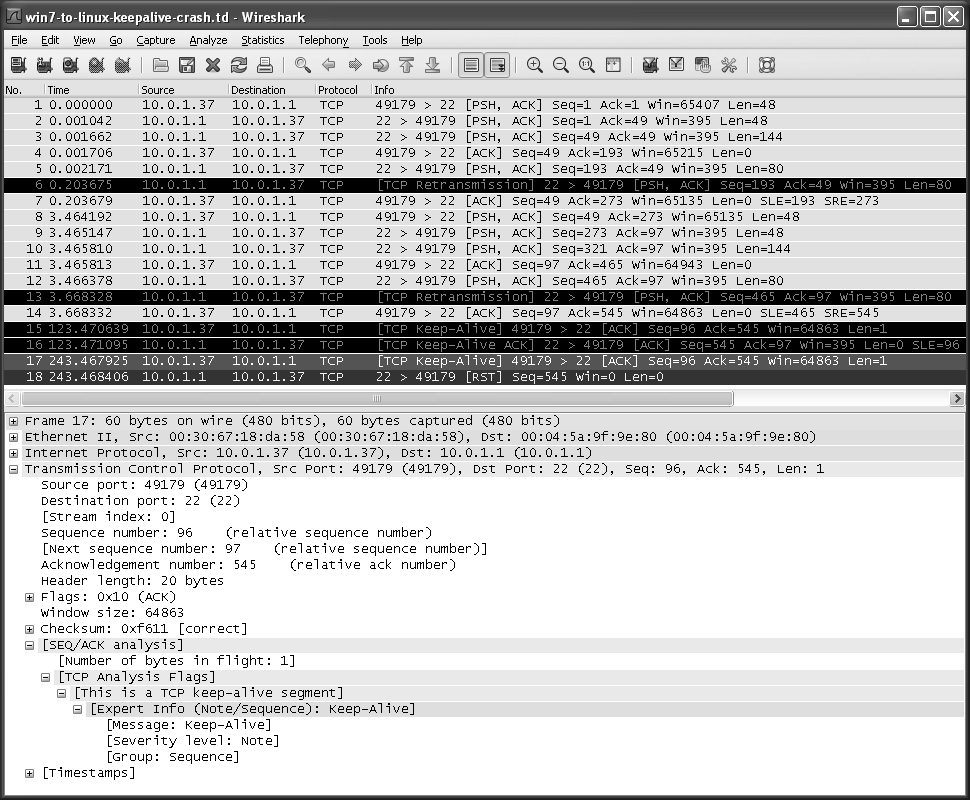
\includegraphics[width=1\textwidth]{imgs/17/17-2.png}
	\caption{在客户端发送保活报文的间隔中,服务器已经重新启动。由于服务器不知道该连接的任何信息,所以返回一个重置报文段}
\end{figure}

\subsubsection{另一端不可达}
在这种情况下,服务器没有崩溃,但是在保活探测报文发送间隔内无法到达。原因可能是中间路由器崩溃,或者会话连接出现故障,或者其他类似的情况。为了模拟这种情况,需
要利用配置了保活功能的 sock 程序与Web 服务器之间建立一条连接。我们使用一台 Mac OSx系统的客户端和一台 LDAP 服务器(端口389),它运行于网站ldap.mit.edu。这里我们缩
短了客户端的保活时间值( 了方便),然后打开连接,之后断开网络连接,然后来看看会有什么影响。下面是命令行和客户端的输出。

\begin{verbatim}
    Mac# Byectl - net.inet.tcp.keepid1e=75000
Mact
sock -k ldap.mit.edu 389
rec error: Operation timed out
about 14 minutes later
\end{verbatim}

图17-3显示了利用 Wireshark 记录的整个过程。

\begin{figure}[!htb]
    \centering
	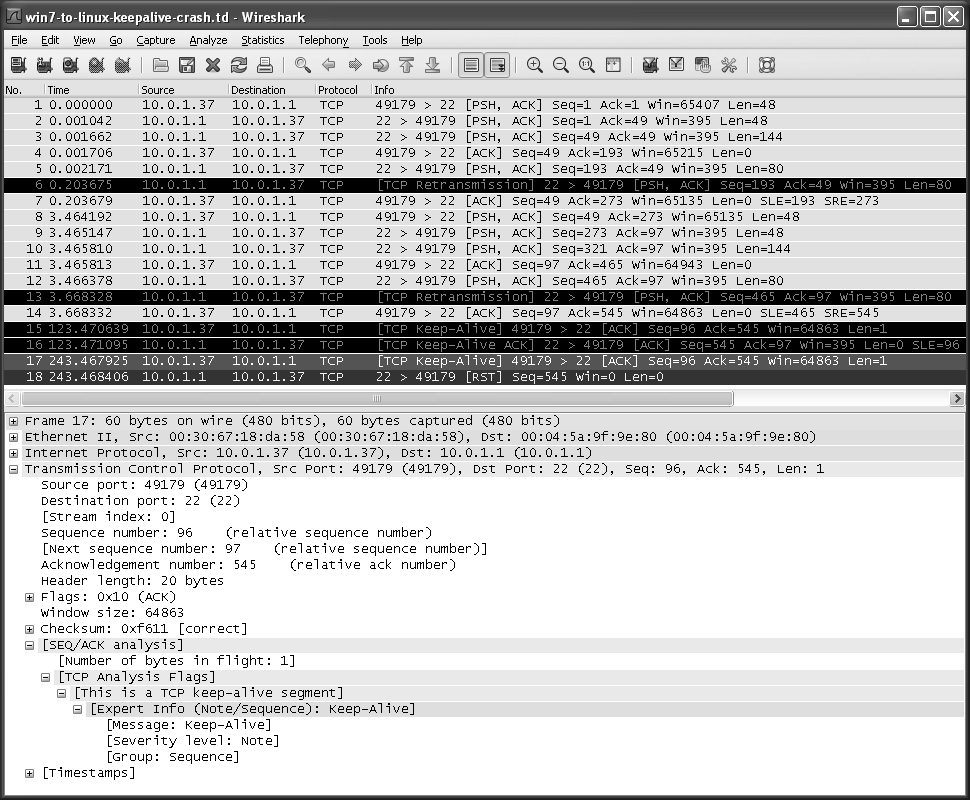
\includegraphics[width=1\textwidth]{imgs/17/17-2.png}
	\caption{第一次保活探測报文被确认之后、网络连接断开。客户端每隔75秒发送出一个新的探测报文。在发送了。次都没有响应之后,连接被断开。同时客户端向对方发送一个重置信号。对
    于客户端而言,这种情况与图17-1所示的眼务器崩溃的情况相同}
\end{figure}

从图中我们可以看到一个完整的连接过程。在初始的三次握手之后,连接保持空闲状态。在大约 75秒时(数据包4)客户端发送一个保活报文并得到确认响应。这个第一次发送
的保活报文是由变量 net.inet:top.keopidle的值来决定的。在这之后不久,网络开始工作。由于连接的两端都没有传输数据,所以在150秒(75秒之后,等于变量 net inet.tcp.keepintvl
的值)时,客户端会发送一个新的保活报文,如数据包7~14所显示的重复操作。虽然服务器开启且正常工作,但是客户端仍然不能接收到任何响应。最后,当客户端第9次发送保
活报文,并且经过75秒之后仍没有收到碗认响应时,客户端结束该连接。连接中断时客户端会向服务器发送一个重置报文段(数据包15)。当然,由于网络是断开的,所以服务器不
能接收到这个数据包。

像上面例子显示的一样,当客户端的 TCP 不能利用保活报文与对方通信时,客户端在终止该连接前还会做一定次数的尝试。这基本上与我们前面看到的另一端主机崩溃的情况相
同。在大多数情况下,发送端不能区分这两种状态。也会有一些例外情况,如通过ICMP 可以知道目的主机不可达,或者由于其他的网络原因导致目的主机不可用。但是由于ICMP 经
常被阻塞,所以很少能区分。因此,TCP 保活机制(或者一些由应用层实现的相似的机制)可以用来检测连接断开的周期。

\section{与TCP 保活机制相关的攻击}
之前提到过,ssh(第2版)中含有一种应用层的保活机制,称为服务器保活报文和客户端保活报文。与TCP 保话报文的区别在于,它们是在应用层通过一条加密的链路传输的,
而且这些报文中包含数据。TCP 保活报文中不包含任何用户数据,所以它最多只进行有限的加密。因此 TCP 保活机制容易受到欺骗攻击。当受到欺骗攻击时,在相当长的一段时间内,
受害主机必须维护不必要的会话资源。

还有一些相对次要的问题。TCP 保活机制的计时器是由之前提到的不同配置参数决定的,而不是用于数据传输的重传计时器。对于被动的观察者来说,他们能够注意到保活报文的有
在,并观察保活报文发送的间隔时间,从而了解系统的配置参数(可能获取发送系统类别信息,称为系统指纹)或者网络的拓扑结构(即下一跳路由器是否能够转发数据流量)。这些问
题在某些环境下是非常重要的。

\section{总结}
如前所述,保活功能存在一定争议性。协议专家仍然在不断争论该功能是否应该属于传输层,还是全部交由应用层处理。现在所有主流TCP版本都实现了保活功能。应用层可以
选择是否开启这一功能来建立连接。开启保活功能,即使在没有应用层数据传输的情况下,仍能帮助服务器判断没有响应的客户端,也可以帮助客户端保持连接活跃性(例如保持 NAT
状态活跃)。

若某个连接长时间处于空闲状态(通常这段时间设定为2小时),在该连接的一端会发送一个探测数据包(虽然这个数据包可以不含任何数据,但通常情况下会包含“垃圾”字节),
从而实现保活功能。可能会发生4种不同的情况:另一端仍在工作;另一端崩溃;另一端崩溃并且已经重新启动;另一端当前无法到达。我们分别举了一个例子来观察这4种情况。

在前两个例子中,如果没有使用保活功能,而且也没有应用层的计时器或者计时器未被激活,那么 TCP 将不会知道另一端已经崩溃(或已经崩溃但已重新启动)。在最后一个例子
中,连接的两端都没有出现差错,而连接最终却被断开了。在使用保活功能的时候,我们必须意识到这一功能的限制,并且考虑这种处理方式是否是我们所期望的。

针对保活机制的攻击主要包括两种:一种是使系统长时间地维护不必要的会话资源,另一种是获得端系统隐藏的一些信息(虽然这些信息对于攻击者而言可能实用性有限)。此外,
由于默认情况下 TCP 不会对保活报文进行加密,所以保活探测报文和确认报文都有可能被利用。然而,对于应用层的保活机制(例如ssh),这些报文都会被加密,所以也就不会出现
上述情况。

\section{参考文献}
[LKA] http://libkeepalive.sourceforge.net
[RFC1122] R. Braden, ed., "Requirements for Internet Hosts," Internet RFC 1122, Oct. 1989.